\section{填写内容}

\begin{frame}[fragile]
\frametitle{Hello world!}
\begin{texcode}[basicstyle=\small\ttfamily, xleftmargin=1.2cm,
    emph={[1]document}, emph={[2]article}]
  % 用 pdfLaTeX、XeLaTeX 或 LuaLaTeX 编译
  \documentclass{article}
  \begin{document}
  Hello world!
  \end{document}
\end{texcode}
\pause
\begin{texcode}[basicstyle=\small\ttfamily, xleftmargin=1.2cm,
    emph={[1]document}, emph={[2]ctexart}]
  % 用 XeLaTeX 或 LuaLaTeX 编译
  \documentclass{ctexart}
  \begin{document}
  你好,世界!
  \end{document}
  \end{texcode}
\end{frame}

\begin{frame}[fragile]
\frametitle{引擎与格式}
\begin{itemize}
  \item<+-> \textbf{引擎}:\TeX{} 的实现

    \begin{itemize}
      \item \pdfTeX{}:直接生成 PDF,支持 micro-typography
      \item \XeTeX{}:支持 Unicode、OpenType 与复杂文字编排(CTL)
      \item \LuaTeX{}:支持 Unicode、OpenType,内联 Lua
      \item (u)p\TeX{}:日本方面推动,生成 |.dvi|,(支持 Unicode)
      \item Ap\TeX{}:底层 CJK 支持,内联 Ruby,Color Emoji(手动斜眼笑)
    \end{itemize}

  \item<+-> \textbf{格式}:\TeX{} 的语言扩展(命令封装)

    \begin{itemize}
      \item plain \TeX{}:Knuth 同志专用
      \item \LaTeX{}:排版科技类文章的事实\zhparen{\textit{de facto}}标准
      \item Con\TeX t:基于 \LuaTeX{} 实现,优雅、易用(吗?)
    \end{itemize}

  \item<+-> \textbf{程序}:引擎 + dump 之后的格式代码

    \begin{itemize}
      \item \alert{英文文章:\pdfLaTeX{}、\XeLaTeX{} 或 \LuaLaTeX{}}
      \item \alert{中文文章:\XeLaTeX{} 或 \LuaLaTeX{}}
    \end{itemize}
\end{itemize}
\end{frame}

\begin{frame}[fragile]
\frametitle{编译}
\begin{itemize}
  \item 现代 \TeX{} 引擎均可直接生成 PDF \pause
  \item 命令行

    \begin{itemize}
      \item |pdflatex|/|xelatex|/|lualatex| + |<文件名>[.tex]|
      \item 多次编译:读取并排版中间文件 \pause
      \item 推荐 \pkg{latexmk}:|latexmk [<选项>] <文件名>|
    \end{itemize} \pause

  \item 编辑器

    \begin{itemize}
      \item 按钮的背后仍然是命令
      \item |PATH| 环境变量:确定可执行文件的位置
      \item VS Code:配置 |tools| 和 |recipes|
    \end{itemize}
\end{itemize}
\end{frame}

\begin{frame}[fragile]
\frametitle{语法}
\begin{itemize}
  \item 注释以 |%| 开头,忽略其后所有内容
  \item 命令以 |\| 开头,区分大小写

    \begin{itemize}
      \item |\foo{arg}|:必选参数放在 |{...}| 中
      \item |\foo[bar]{arg}|:可选参数放在 |[...]|
    \end{itemize}

  \item 环境

    \begin{texcode}[gobble=4, emph={[1]env}]
      \begin{env}
        ...
      \end{env}
    \end{texcode}

  \item 特殊符号需要转义:|\%|、|\$|、|\&|、|\textbackslash| 等
  \item 连续多个空格 = 单个空格 = 单个换行符 \pause
  \item \TeX{}/\LaTeX{} 的语法可以修改
\end{itemize}
\end{frame}

\begin{frame}[fragile]
\frametitle{文件结构}
\begin{texcode}[basicstyle=\scriptsize\ttfamily, moretexcs={\keyword,\boldsymbol},
    emph={[1]document}, emph={[2]article,amsmath}]
  % 用 UTF-8 编码,命名为 xxx.tex
  \documentclass{article}                     % 指明文档类型:文章
  % 导言区:设置文档样式
  \usepackage{amsmath}                        % 调用宏包,实现各种功能
  \newcommand\keyword[1]{\textbf{#1}}         % 自定义命令

  \begin{document}
  % 正文:套用格式
  In quantum mechanics, the \keyword{Schr\"odinger equation} is a
  mathematical equation that describes the changes over time of a
  physical system in which quantum effects, such as \keyword{wave--%
  particle duality}, are significant.

  % 上面的空行表示分段
  In classical mechanics, Newton's second law
  ($\boldsymbol{F}=m\boldsymbol{a}$) is used to make a\ldots{}

  Time-dependent Schrödinger equation can be written as  % ö 也能直接用
  \[ i\hbar \frac{d}{dt} |\Psi(t)\rangle = \hat{H} |\Psi(t)\rangle. \]
  \end{document}
\end{texcode}
\vspace{-0.6cm}
\end{frame}

\begin{frame}{Schrödinger equation}
In quantum mechanics, the \textbf{Schr\"odinger equation} is a
mathematical equation that describes the changes over time of a
physical system in which quantum effects, such as \textbf{wave--%
particle duality}, are significant.

In classical mechanics, Newton's second law
($\mathbfit{F}=m\mathbfit{a}$) is used to make a\ldots{}

Time-dependent Schrödinger equation can be written as
\[ i\hbar \frac{d}{dt} \vert\Psi(t)\rangle = \hat{H} \, \vert\Psi(t)\rangle. \]
\end{frame}

\begin{frame}[fragile]
\frametitle{谋篇布局}
\begin{itemize}
  \item 文档部件

    \begin{itemize}
      \item 标题:|\title|、|\author|、|\date| $\to$ |\maketitle|
      \item 摘要:|abstract| 环境
      \item 目录:|\tableofcontents|
      \item 章节:|\chapter|、|\section|、|\subsection| 等
      \item 文献:|\bibliography|
    \end{itemize}

  \item 文档划分

    \begin{itemize}
      \item 凤头猪肚豹尾:|\frontmatter|、|\mainmatter|、|\backmatter|
      \item 分文件编译:|\include|、|\input|
    \end{itemize}
\end{itemize}
\end{frame}

\begin{frame}[fragile]
\frametitle{文本标记(一)}
\begin{itemize}
  \item 加粗:|{\bfseries ...}| 或 |\textbf{...}|
  \item 倾斜:|{\itshape ...}| 或 |\textit{...}|
  \item 字号:|\tiny|、|\small|、|\large|、|\Large| 等
  \item 换行:|\\|
  \item 缩进:|\indent|
  \item 居中:|\centering| 或 |center| 环境
\end{itemize}
\end{frame}

\begin{frame}[standout]
  \huge \textbf{请忘记上一页}
\end{frame}

\begin{frame}[fragile]
\frametitle{文本标记(二)}
\begin{itemize}
  \item 为什么要有不同的标记?\pause\mbox{}——表达不同的\alert{语义} \pause
  \item |\textbf| 这样的命令是否表达语义? \pause
  \item 再提一遍基本原则:\alert{内容与格式分离} \pause
  \item 正确(或曰:合理)的做法

    \begin{itemize}
      \item 强调文字(意大利体):|\emph{...}|
      \item 摘要(居中,小字号,带有标题):|abstract| 环境
      \item 引用(左右边距较大):|quote| 或 |quotation| 环境
      \item 自定义新的命令、环境
    \end{itemize} \pause

  \item 报告,我想偷懒!
\end{itemize}
\end{frame}

\begin{frame}[fragile]
\frametitle{常用环境:列表与枚举}
\begin{columns}
\begin{column}{0.55\textwidth}
  \begin{texcode}[gobble=4, emph={[1]enumerate,itemize}]
    \begin{enumerate}
      \item Da Vinci
        \begin{itemize}
          \item \textit{The Last Supper}
          \item \textit{Salvator Mundi}
          \item \textit{Mona Lisa}
        \end{itemize}
      \item Shakespeare
        \begin{itemize}
          \item \textit{Macbeth}
          \item \textit{Hamlet}
          \item \textit{King Lear}
          \item \textit{Othello}
        \end{itemize}
    \end{enumerate}
  \end{texcode}
\end{column}
\pause
\begin{column}{0.35\textwidth}
  \begin{enumerate}
    \item Da Vinci
      \begin{itemize}
        \item \textit{The Last Supper}
        \item \textit{Salvator Mundi}
        \item \textit{Mona Lisa}
      \end{itemize}
    \item Shakespeare
      \begin{itemize}
        \item \textit{Macbeth}
        \item \textit{Hamlet}
        \item \textit{King Lear}
        \item \textit{Othello}
      \end{itemize}
  \end{enumerate}
\end{column}
\end{columns}
\end{frame}

\begin{frame}[fragile]
\frametitle{常用环境:图片}
\begin{columns}
\begin{column}{0.6\textwidth}
  \begin{texcode}[gobble=4, moretexcs={\graphicspath,\includegraphics},
      emph={[1]figure}, emph={[2]graphicx}]
    % 不是 graphics
    \usepackage{graphicx}
    % 可以统一指定图片路径
    \graphicspath{{./images/}}

    \begin{figure}
      \centering
      % 可指定宽度、高度等选项
      \includegraphics[...]{fudan-logo.pdf}
      \caption{Logo of Fudan University}
      \label{fig:fudan-logo}
    \end{figure}
  \end{texcode}
\end{column}
\pause
\begin{column}{0.3\textwidth}
  \begin{figure}
    \centering
    \fduemblem+[x=0.1pt, y=0.1pt, color=FudanBlue]
    \caption{\textcolor{keyword}{Figure \thefigure:} Logo of Fudan University}
    \label{fig:fudan-logo_}  % Avoid duplicate labels warning
  \end{figure}
\end{column}
\end{columns}
\end{frame}

\begin{frame}[fragile]
\frametitle{常用环境:表格}
\begin{columns}
\begin{column}{0.6\textwidth}
  \begin{texcode}[gobble=4, moretexcs={\toprule,\midrule,\bottomrule},
      emph={[1]table,tabular}, emph={[2]booktabs}]
    \usepackage{booktabs} % 三线表
    \begin{table}
      \caption{Population Census of China}
      \label{tab:china-population}
      % 列格式:c 居中,l 左对齐,r 右对齐
      \begin{tabular}{cc}
        \toprule
          Year & Population \\
        \midrule
          1953 &  6.0 \\
          ...
          2020 & 14.1 \\
        \bottomrule
      \end{tabular}
    \end{table}
  \end{texcode}
\end{column}
\pause
\begin{column}{0.3\textwidth}
  \begin{table}
    \caption{\textcolor{keyword}{Table \thetable:} Population Census of China}
    \label{tab:china-population_}
    \footnotesize
    \begin{tabular}{cc}
      \toprule
        Year & Population \\
      \midrule
        1953 &  6.0 \\
        1964 &  6.9 \\
        1982 & 10.1 \\
        1990 & 11.3 \\
        2000 & 12.7 \\
        2010 & 13.4 \\
        2020 & 14.1 \\
      \bottomrule
    \end{tabular}
  \end{table}
\end{column}
\end{columns}
\end{frame}

\begin{frame}[fragile]
\frametitle{常用环境:定理}
\begin{columns}
\begin{column}{0.57\textwidth}
  \begin{texcode}[gobble=4, moredelim={[is][emphstyle]{!}{!}}, moretexcs={\newtheorem*},
      emph={[2]amsthm}]
    \usepackage{amsthm}
    % 需要预先定义
    \newtheorem{theorem}{Theorem}
    \newtheorem*{remark}{Remark} % 不编号

    \begin{!theorem!}[Fermat]
      $a^n+b^n=c^n$ has no positive...
    \end{!theorem!}
    \begin{!proof!}
      % 证明后面会有 QED 符号
      It's obvious.
    \end{!proof!}
    \begin{!remark!}
      The cases $n=1$ and $n=2$...
    \end{!remark!}
  \end{texcode}
\end{column}
\pause
\begin{column}{0.33\textwidth}
  \footnotesize
  \setlength{\parskip}{0.5em}
  \setlength{\parindent}{0pt}

  \textbf{Theorem 1} (Fermat). \emph{$a^n+b^n=c^n$ has no positive integer solutions
    for $x$, $y$ and $z$ when $n$ is greater than 2.}

  \textit{Proof.} It's obvious. \hfill $\mdlgwhtsquare$

  \textbf{Remark.} \emph{The cases $n=1$ and $n=2$ have been known since antiquity
    to have infinitely many solutions.}
\end{column}
\end{columns}
\end{frame}

\begin{frame}[fragile]
\frametitle{浮动体与交叉引用}
\begin{itemize}
  \item<+-> 浮动体机制

    \begin{itemize}
      \item |figure| 和 |table| 环境
      \item 文本为主,图、表为辅
      \item 希望浮动体不要乱跑:「这是病,得治」
            \link{https://liam.page/2017/03/11/floats-in-LaTeX-basic}
      \item 避免「见上图」、「见下表」
      \item 建议写完全文之后统一调整
    \end{itemize}

  \item<+-> 以标签控制交叉引用

    \begin{itemize}
      \item 被引处:|\label|
      \item 引用处:|\ref|、|\eqref| 等(如图~\textcolor{emph1}{\ref{fig:fudan-logo_}}、
            表~\textcolor{emph1}{\ref{tab:china-population_}})
      \item 用有意义的标签:|\label{eq:euler-lagrange-eq}|
      \item 需多次编译——推荐 \pkg{latexmk}
    \end{itemize}
\end{itemize}
\end{frame}

\begin{frame}[fragile]
\frametitle{如何在论文中画出漂亮的插图?}
\begin{itemize}
  \item<+-> 外部插入

    \begin{itemize}
      \item Mathematica、MATLAB
      \item PowerPoint、Visio、Adobe Illustrator、Inkscape
      \item Python \texttt{Matplotlib}、\texttt{Plots.jl}、R、Plotly 等
      \item draw.io \link{https://www.draw.io}、
            Mathcha \link{https://www.mathcha.io}、
            ProcessOn \link{https://www.processon.com} 等网站
    \end{itemize}

  \item<+-> \TeX{} 内联

    \begin{itemize}
      \item Asymptote
      \item \alert{\pkg{pgf}/\pkg{TikZ}、\pkg{pgfplots}}
    \end{itemize}

  \item<+-> 插图格式

    \begin{itemize}
      \item 矢量图:|.pdf|
      \item 位图:|.jpg| 或 |.png|
      \item \alert{不再推荐 \texttt{.eps}}
      \item 不(完全)支持 |.svg|、|.bmp|
    \end{itemize}

  \item<+-> 参考:\link{https://www.zhihu.com/question/21664179}
                  \link{https://tex.stackexchange.com/q/158668}
                  \link{https://tex.stackexchange.com/q/72930}
\end{itemize}
\end{frame}

\begin{frame}[fragile]
\frametitle{文献}
\begin{itemize}
  \item 建议自动生成\pause (你只有三篇参考文献?)\pause
  \item |.bib| 数据库(条目会包含 key,用于引用)

    \begin{itemize}
      \item Google Scholar 复制,Zotero、Jabref 等生成
      \item 注意特殊符号、公式等常常需要人工检查
    \end{itemize} \pause

  \item 传统方法:\BibTeX{} 后端

    \begin{itemize}
      \item 指定样式:|\bibliographystyle{<style>}|(导言区)
      \item 标记引用:|\cite{<key>}|
      \item 插入参考文献:|\bibliography{<bib 文件>}|
      \item 更多文献、引用样式:\pkg{natbib} 宏包
      \item 国家标准 GB/T 7714--2015
            \link{https://www.gb688.cn/bzgk/gb/newGbInfo?hcno=7FA63E9BBA56E60471AEDAEBDE44B14C}
            \link{https://github.com/Haixing-Hu/GBT7714-2005-BibTeX-Style/files/153951/GBT.7714-2015.pdf}:
            \alert{\pkg{gbt7714} 宏包}
    \end{itemize} \pause

  \item 现代方法:\pkg{biber} 后端 + \pkg{biblatex} 宏包

    \begin{itemize}
      \item 国家标准:\pkg{biblatex-gb7714-2015} 宏包
    \end{itemize} \pause

  \item 需多次编译——再次推荐 \pkg{latexmk}
\end{itemize}
\end{frame}

\begin{frame}[standout]
  \begingroup
    \xeCJKsetup{xeCJKactive=false}
    \SourceHanSerifNoCJK\fontsize{72}{84}\selectfont
    ⿺辶⿳穴⿰月⿰⿲⿱幺長⿱言馬⿱幺長刂心
  \endgroup \\[2ex]
  \footnotesize \texttt{U+30EDE}
\end{frame}

\begin{frame}{中文支持}
\begin{columns}
\begin{column}{0.66\textwidth}
  \begin{itemize}
    \item 中文有什么特殊?\pause

      \begin{itemize}
        \item 汉字太多(92,856+)\pause
        \item 横排 + 直排、标点禁则、行间注 \link{https://www.w3.org/TR/clreq} \pause
        \item \jatext{にほんご}、
              {\NotoDevanagari देवनागरी}、
              {\NotoArabic العَرَبِيَّة‎}、
              {\NotoEgyptian 𓅡𓎡𓅱𓀀𓏪}
      \end{itemize} \pause

    \item 已淘汰:

      \begin{itemize}
        \item CCT 系统、\pkg{CJK} 宏包(裸用)
        \item \CTeX{} 套装
      \end{itemize} \pause

    \item 目前推荐手段:

      \begin{itemize}
        \item \alert{\pkg{ctex} 宏集}(此 \pkg{ctex} 非彼 \CTeX{})
        \item \XeLaTeX{} 编译
      \end{itemize} \pause

    \item 可以用,不推荐:

      \begin{itemize}
        \item \pkg{xeCJK} 宏包(裸用)
        \item \pkg{ctex} 宏集 + 其他引擎编译
      \end{itemize}
  \end{itemize}
\end{column} \pause
\begin{column}{0.32\textwidth}
  \tiny
  \begin{tabular}{cc}
    
\includegraphics[width=24pt]{figures/leoliu.png}        &
    
\includegraphics[width=24pt]{figures/qinglee.jpg}       \\
    刘海洋 & 李清 \\[2ex]
    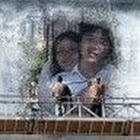
\includegraphics[width=24pt]{figures/wulingyun.jpg}     &
    
\includegraphics[width=24pt]{figures/jjgod.jpg}         \\
    吴凌云 & 江疆 \\[2ex]
    
\includegraphics[width=24pt]{figures/li-a-ling.jpg}     &
    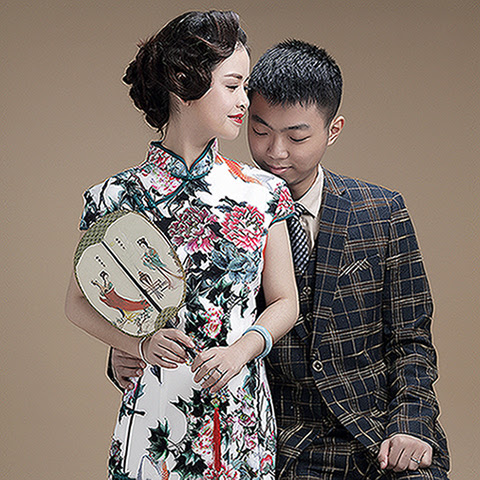
\includegraphics[width=24pt]{figures/liam-huang.jpg}    \\
    马起园 & 黄晨成 \\[2ex]
    
\includegraphics[width=24pt]{figures/louisstuart96.jpg} &
    
\includegraphics[width=24pt]{figures/zepinglee.jpg}     \\
    鲁尚文 & 李泽平 \\[2ex]
    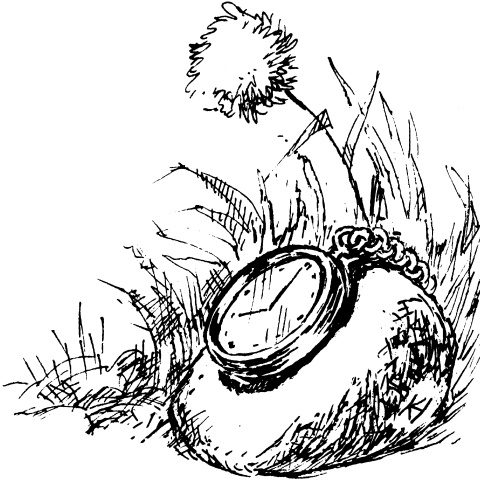
\includegraphics[width=24pt]{figures/muzimuzhi.jpg}     &
    
\includegraphics[width=24pt]{figures/ruixi-zhang.png}   \\
    周宇恺 & 张瑞熹
  \end{tabular}
  \vspace{-0.6cm}
\end{column}
\end{columns}
\nonumberfootnote[<8->]{图片来源:GitHub、Twitter、知乎}
\end{frame}

\begin{frame}[fragile]
\frametitle{模板}
\begin{itemize}
  \item<+-> 是什么?

    \begin{itemize}
      \item 设计好的格式框架
      \item 专注于内容:\alert{不要追求与期刊排版一致}
      \item Word 中的样式:「学好 \LaTeX{} 可以更科学地使用 Word」
    \end{itemize}

  \item<+-> 有哪些?

    \begin{itemize}
      \item 期刊:\pkg{revtex}、\pkg{elsarticle}、\pkg{IEEEtran}……
      \item 学位论文:\pkg{thuthesis}、\pkg{ustcthesis}、\alert{\pkg{fduthesis}}……
    \end{itemize}

  \item<+-> 怎么用?

    \begin{itemize}
      \item |\documentclass{...}|,配置参数,照常编写
      \item \alert{看文档,看文档,看文档}
    \end{itemize}

  \item<+-> 去哪里找?

    \begin{itemize}
      \item CTAN \link{https://ctan.org} 或 GitHub \href{https://github.com}{\faGithub}
      \item 期刊官网
      \item 「湿兄用 U 盘拷给你的模板一定是过时的」
    \end{itemize}
\end{itemize}
\end{frame}

\begin{frame}[fragile]
\frametitle{幻灯片}
\begin{itemize}
  \item<+-> 基本框架

    \begin{itemize}
      \item \pkg{beamer} 或 \pkg{ctexbeamer} 文档类
      \item 页面由 |frame| 环境组织
      \item 文本内容:建议使用 |itemize| 和 |enumerate|
      \item 图表:不再浮动,不建议使用交叉引用
      \item 定理及强调:|theorem|、|proof|、|block| 等
      \item 分栏:|columns| + |column| 环境
    \end{itemize}

  \item<+-> 主题与样式

    \begin{itemize}
      \item |\usetheme|、\lstinline[style=style@inline]+\use[font|color|inner|outer]theme+
      \item 更现代的主题:|metropolis|
      \item 使用「默认」字体:|\usefonttheme{serif}|
    \end{itemize}

  \item<+-> 动画(覆盖)

    \begin{itemize}
      \item |\pause| 命令
      \item |\onslide<1>|、|\item<1+>| 等
    \end{itemize}
\end{itemize}
\end{frame}
